\documentclass{article}

\usepackage{graphicx}
\usepackage{tikz}
\usepackage{tikzsymbols}
\usetikzlibrary{calc,patterns,shapes.geometric}
\pagestyle{empty}
\usepackage[margin=0pt]{geometry}
\geometry{papersize={14in,12in}}

\def\centerarc[#1](#2)(#3:#4:#5){\draw[#1] ($(#2)+({#5*cos(#3)},{#5*sin(#3)})$) arc (#3:#4:#5);}

\begin{document}
	\begin{figure}
		\centering
		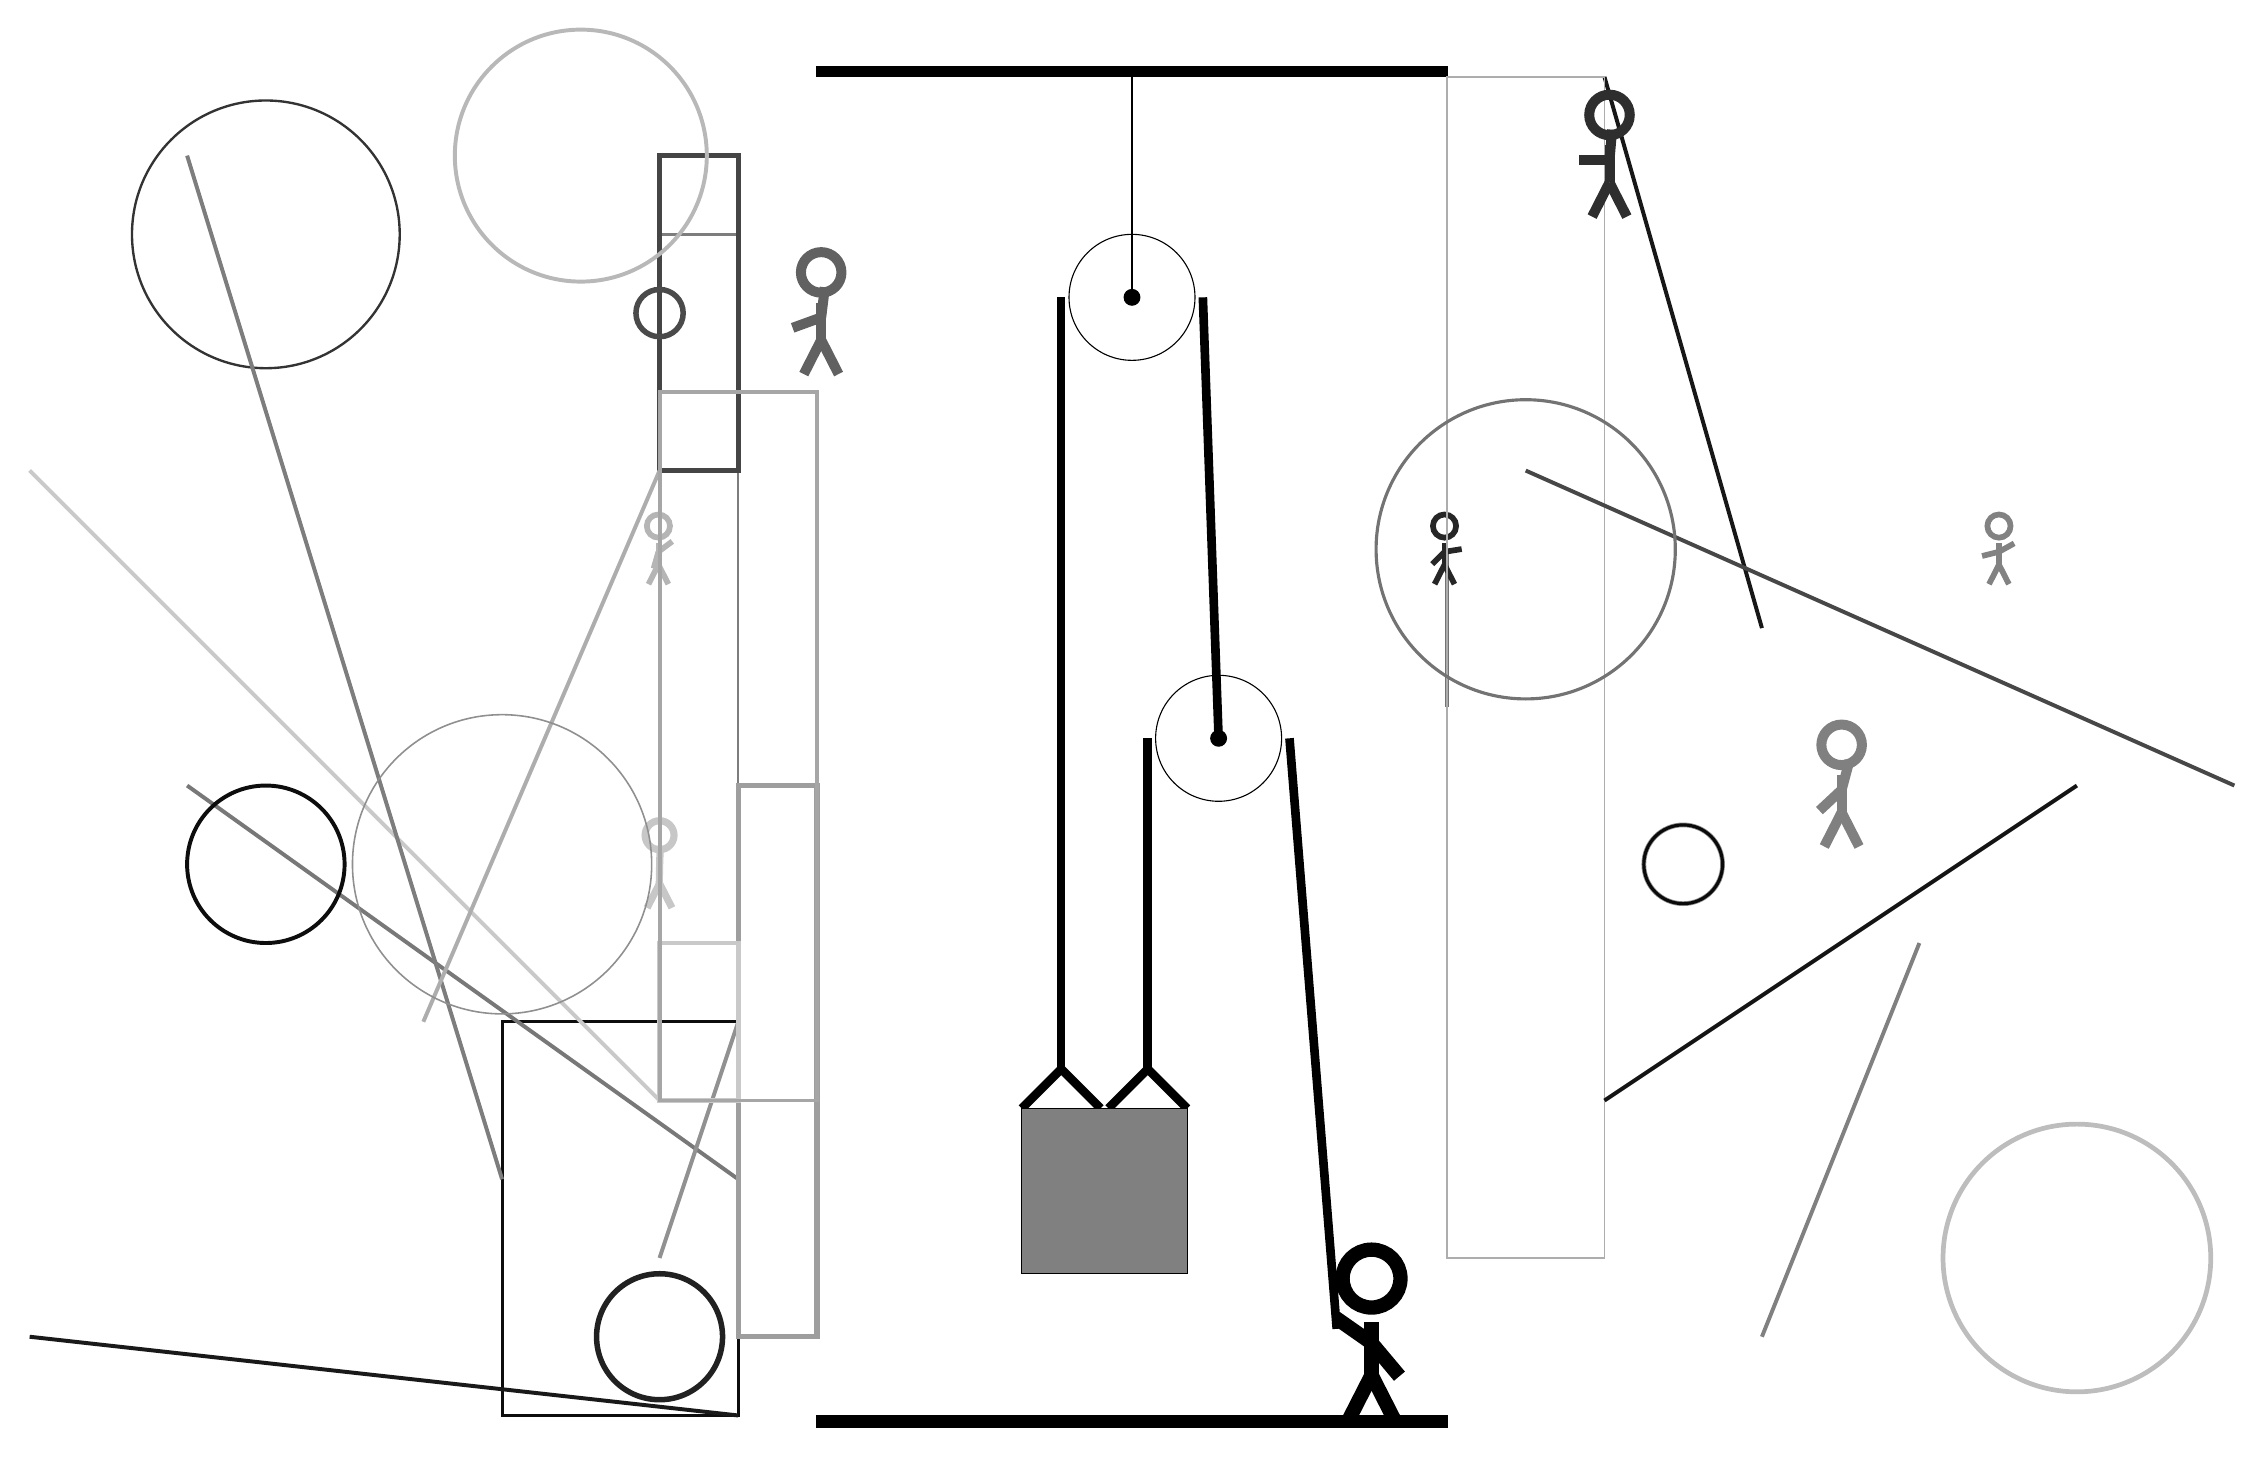
\begin{tikzpicture}
			%%%%% START %%%%%
			
			\draw[fill=black] (-2, 14) rectangle (6, 14.125);
			
			\draw (2, 11.2) circle (0.8);
			\draw[fill=black] (2, 11.2) circle (0.1);
			\draw[thick] (2, 11.2) -- (2, 14);
			
			\draw (3.1, 5.6) circle (0.8);
			\draw[fill=black] (3.1, 5.6) circle (0.1);
			
			\draw[line width = 1.1mm]  (0.6, 0.9) -- (1.1, 1.4) -- (1.6, 0.9);
			\draw[line width = 1.1mm]  (1.7, 0.9) -- (2.2, 1.4) -- (2.7, 0.9);
			\draw[fill=black!50] (0.6, 0.9) rectangle (2.7, -1.2);
			
			\draw[line width=0.4mm, color=black!55] (6, 6) rectangle (6, 8);
			
			\draw [line width=0.3mm, color=black!80](-9, 12) circle (1.7);
			\draw[line width=0.4mm, color=black!95] (-3, -3) rectangle (-6, 2);
			\node[line width=0.6mm, color=black!22] at (-4, 4) {\Strichmaxerl[5][89][88]};
			
			\draw[line width=0.5mm, color=black!90](-3, -3) -- (-12, -2);
			
			\draw [line width=0.6mm, color=black!26](14, -1) circle (1.7);
			\node[line width=0.4mm, color=black!85] at (6, 8) {\Strichmaxerl[4][45][9]};
			\draw[line width=0.5mm, color=black!21](-4, 1) -- (-12, 9);
			\draw[line width=0.3mm, color=black!51] (-4, 3) rectangle (-3, 12);
			\draw[line width=0.5mm, color=black!53](-3, 0) -- (-10, 5);
			
			\draw [line width=0.5mm, color=black!95](-9, 4) circle (1.0);
			\draw [line width=0.6mm, color=black!44](9, 4) circle (0.5);
			\draw [line width=0.7mm, color=black!87](-4, -2) circle (0.8);
			
			\draw[line width=0.7mm, color=black!73] (-4, 9) rectangle (-3, 13);
			\draw[line width=0.5mm, color=black!50](10, -2) -- (12, 3);
			\draw[line width=0.5mm, color=black!51](-6, 0) -- (-10, 13);
			
			\draw[line width=0.5mm, color=black!32](-4, 9) -- (-7, 2);
			\draw[line width=0.5mm, color=black!43](-4, -1) -- (-3, 2);
			\draw [line width=0.7mm, color=black!71](-4, 11) circle (0.3);
			\node[line width=0.7mm, color=black!50] at (11, 5) {\Strichmaxerl[7][43][75]};
			\draw [line width=0.2mm, color=black!44](-6, 4) circle (1.9);
			
			\node[line width=0.4mm, color=black!29] at (-4, 8) {\Strichmaxerl[4][74][37]};
			
			\draw[line width=0.5mm, color=black!91](10, 7) -- (8, 14);
			\node[line width=0.3mm, color=black!62] at (-2, 11) {\Strichmaxerl[7][20][83]};
			\draw [line width=0.5mm, color=black!28](-5, 13) circle (1.6);
			
			\draw[line width=0.7mm, color=black!38] (-3, -2) rectangle (-2, 5);
			\draw[line width=0.6mm, color=black!21] (-4, 1) rectangle (-3, 3);
			\draw[line width=0.2mm, color=black!32] (6, -1) rectangle (8, 14);
			\node[line width=0.4mm, color=black!49] at (13, 8) {\Strichmaxerl[4][14][29]};
			\draw[line width=0.5mm, color=black!72](7, 9) -- (16, 5);
			\draw[line width=0.5mm, color=black!92](8, 1) -- (14, 5);
			
			\draw [line width=0.4mm, color=black!96](9, 4) circle (0.5);
			\draw[line width=0.5mm, color=black!35] (-2, 10) rectangle (-4, 1);
			\draw [line width=0.4mm, color=black!55](7, 8) circle (1.9);
			
			\node[line width=0.7mm, color=black!82] at (8, 13) {\Strichmaxerl[7][0][85]};
			
			\draw[line width = 1.1mm] (1.1, 11.2) -- (1.1, 1.4);
			\centerarc[line width = 1.1mm](2, 11.2)(0:180:0.9);
			\draw[line width = 1.1mm] (2.9, 11.2) -- (3.1, 5.6);
			\draw[line width = 1.1mm] (2.2, 5.6) -- (2.2, 1.4);
			\centerarc[line width = 1.1mm](3.1, 5.6)(0:180:0.9);
			\draw[line width = 1.1mm] (4.0, 5.6) -- (4.6, -1.9);
			
			\node at (5, -2) {\Strichmaxerl[10][-35][-50]};
			
			\draw[fill=black] (-2, -3) rectangle (6, -3.15);
			
			%%%%% END %%%%%
		\end{tikzpicture}
	\end{figure}	
\end{document}